\chapter{Appendix} \label{sec:appendix}

\section{Chapter 7}
\subsection{Low-rank Approximation}\label{Appendix low rank}
Here we show our preliminery results on the employed low-rank approximation of confusion matrices for BraTS dataset, precluded in the main text. Table.~\ref{low_rank_result} compares the performance of our method with the default implementation and the one with rank-1 approximation. We see that the low-rank approximation can halve the number of parameters in CMs and the number of floating-point-operations (FLOPs) in computing the annotator prediction while resonably retaining the performance on both segmentation and CM estimation. We note, however, the practical gain of this approximation in this task is limited since the number of classes is limited to 4 as indicated by the marginal reduction in the overall GPU usage for one example. We expect the gain to increase when the number of classes is larger as shown in Fig.~\ref{fig:low_rank_complexity}. 

\begin{table}[H]
	\center
	\footnotesize
	\begin{tabular}{@{}llllll}
		\hline
		 Rank & Dice & CM estimation & GPU Memory & No. Parameters &  FLOPs   \\
		\hline	
		Default  & 53.47 $\pm $ 0.24  & 0.1185 $\pm$ 0.0056   & 2.68GB &  589824 &  1032192  \\
		rank 1 & 50.56 $\pm$ 2.00  & 0.1925 $\pm$ 0.0314 & 2.57GB  &    294912    & 405504\\
		\hline
	\end{tabular}%
	\vspace{2mm}
\caption{\footnotesize Comparison between the default implementation and low-rank (=1) approximation on BraTS. GPU memory consumption is estimated for the case with batch size = 1. Bot the total number of variables in the confusion matrices, and the number of FLOPs required in computing the annotator predictions. }
\label{low_rank_result}
\end{table}

Lastly, we also describe the details of the devised low-rank approximation. Analogous to Chandra and Kokkinos's work \cite{chandra2017dense} where they employed a similar approximation for estimating the pairwise terms in densely connected CRF,  we parametrise the spatial CM, $\hat{\textbf{A}}_{\phi}^{(r)}(\textbf{x}) = \textbf{B}_{1, \phi}^{(r)}(\textbf{x})\cdot\textbf{B}^{T,(r)}_{2, \phi}(\textbf{x})$ as a product of two smaller rectangular matrices $\textbf{B}_{1, \phi}^{(r)}$ and $\textbf{B}_{2, \phi}^{(r)}$ of size $W\times H \times L \times l$ where $l << L$. In this case, the annotator network outputs $\textbf{B}_{1, \phi}^{(r)}$ and $\textbf{B}_{2, \phi}^{(r)}$ for each annotator in lieu of the full CM. Two separate rectangular matrices are used here since the confusion matrices are not necessarily symmetric. Such low-rank approximation reduces the total number of variables to $2WHLl$ from $WHL^2$ and the number of floating-point operations (FLOPs) to $WH(4L(l - 0.25) - l)$ from $WH(2L-1)L$. Fig.~\ref{fig:low_rank_complexity} shows that the time and space complexity of the default method grow quadratically in the number of classes while the low-rank approximations have linear growth. 

\begin{figure}[H]
    \centering
    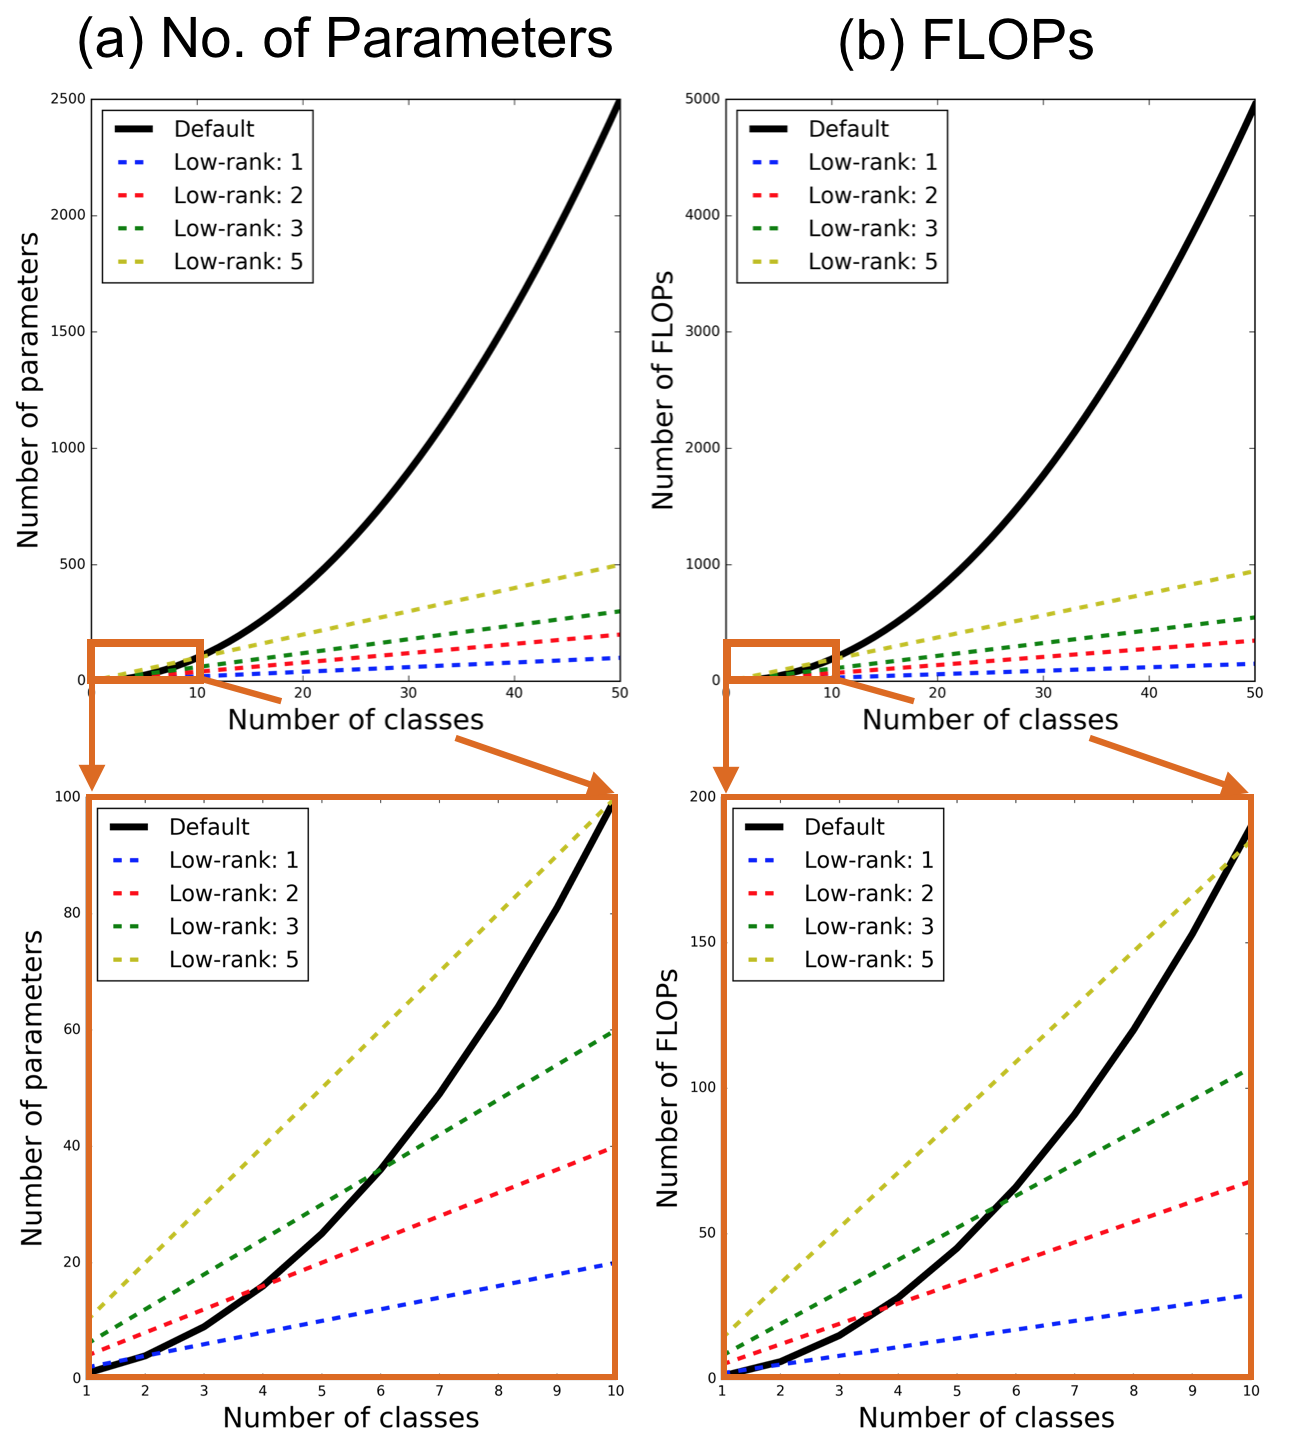
\includegraphics[width=0.5\linewidth]{chapter_8_neurips/picture20.png}
    %\addtocounter{figure}{+1}
    \caption{\footnotesize Comparison of time and space complexity between the default implementation and the low-rank counterparts. (a) compares the number of parameters in the confusion matrices while (b) shows the number of FLOPs required to compute the annotator predictions (the product between the confusion matrices and the estimated true segmentation probabilities).}
    \label{fig:low_rank_complexity}
\end{figure}



\subsection{Proof of Theorem~\ref{theorem:main}}

We first show a specific case of Theorem~\ref{theorem:main} when there is only a single annotator, and subsequently extend it to the scenario with multiple annotators. Without loss of generality, we show the result for an arbitrary choice of a pixel in a given input image $\mathbf{x} \in \mathbb{R}^{W\times H \times C}$. Specifically, let us denote the estimated confusion matrix (CM) of the annotator at the $(i, j)^{\text{th}}$ pixel by $\hat{\textbf{A}} := [\hat{\textbf{A}_\phi}(\mathbf{x})_{ij}] \in [0, 1]^{L\times L}$, and suppose the true class of this pixel is $k \in [1, ...,L]$ i.e., $\textbf{p}(\textbf{x}) = \mathbf{e}_k$ where $\mathbf{e}_k$ denotes the $k^{\text{th}}$ elementary basis. Let $\hat{\textbf{p}}_\theta(\textbf{x})$ denote the $L$-dimensional estimated label distribution at the corresponding pixel (instead of over all the whole image). 
\vspace{3mm}
\begin{lemma}\label{lemma:1}
  If the annotator's segmentation probability is fully captured by the model for the $(i, j)^{\text{th}}$ pixel in image $\mathbf{x}$ i.e., $\hat{\textbf{A}}\cdot \hat{\textbf{p}}_\theta(\textbf{x})=\textbf{A}\cdot \textbf{p}(\textbf{x}) $, and both $\hat{\textbf{A}}$, $\textbf{A}$ satisfy that $a_{kk} > a_{kj}$ for $j \neq k$ and $\hat{a}_{ii} > \hat{a}_{ij}$ for all $i, j$ such that $j \neq i$, then $\text{tr}(\hat{\textbf{A}})$ is minimised when $\hat{\textbf{A}}=\textbf{A}$. Furthermore, if $\text{tr}(\hat{\textbf{A}})=\text{tr}(\textbf{A})$, then the true label is fully recovererd i.e., $ \hat{\textbf{p}}_\theta(\textbf{x}) = \textbf{p}(\textbf{x})$ and the $k^{\text{th}}$ column in $\hat{\textbf{A}}$, $\textbf{A}$ are the same. 
  
  % \textcolor{green}{This last sentence is a bit confusing to a first time reader; We are saying we want diagonal dominant matrices with minimal trace.}. %(\textcolor{red}{diagonally dominant matrices are non-singular by the Levy-Desplanques theorem, thus, sufficient to impose this condition?})
\end{lemma}

\begin{proof}
We first show that the $k^{\text{th}}$ diagonal element in $\textbf{A}$ is smaller than or equal to its estimate in $\hat{\textbf{A}}$. Since $\textbf{p}(\textbf{x}) = \mathbf{e}_k$ is a one-hot vector, $\hat{\textbf{A}}\cdot \hat{\textbf{p}}_\theta(\textbf{x})=\textbf{A}\cdot \textbf{p}(\textbf{x}) $ holds and $\hat{a}_{kk} > \hat{a_{kj}} \forall j \neq k$, it follows that: 
% \begin{equation}
%     tr(\textbf{A}) = tr(\hat{\textbf{A}}\textbf{P}) = \sum_{i,j} \hat{a}_{ij}p_{ji} \leq \sum_{i,j}\hat{a}_{ii}p_{ji} = \sum_{i}\hat{a_{ii}}(\sum_{j}p_{ji}) = \sum_{i}\hat{a}_{ii} = tr(\hat{\textbf{A}})
% \end{equation}
\begin{align}\label{eq:side1}
    a_{kk} &= \Big{\langle} [\hat{a}_{k1},...,\hat{a}_{kL}], \ \ \hat{\textbf{p}}_\theta(\textbf{x}) \Big{\rangle} \\
    &\leq \Big{\langle} [\hat{a}_{kk}, ...,\hat{a}_{kk}], \ \ \hat{\textbf{p}}_\theta(\textbf{x})\Big{\rangle} = \hat{a}_{kk}. \label{eq:trace_inequality}
\end{align}
The possibility of equality in the above comes from the fact that all entries in $\hat{\textbf{p}}_\theta(\textbf{x})$ except the $k$th element could be zeros. Now, the assumption that there is a single ground truth label $k$ for the $(i, j)^{\text{th}}$ pixel means that all the values of the true CM, $\textbf{A}$ are uniformly equal to $1/L$ except the $k^{\text{th}}$ column. In addition, since the diagonal dominance of the estimated CM means each $\hat{a}_{ii}$ is at least $1/L$, we have that 
\begin{align*}
    \text{tr}(\textbf{A}) = \frac{L-1}{L} + a_{kk} \,\leq\,  \sum_{j\neq k}\hat{a}_{jk}  + \hat{a}_{kk} =  \text{tr}(\hat{\textbf{A}}).
\end{align*}

It therefore follows that when $\hat{\textbf{A}} = \textbf{A}$ holds, the trace of $\text{tr}(\hat{\textbf{A}})$ is the smallest. Now, we show that when this holds i.e., $\text{tr}(\textbf{A})= \text{tr}(\hat{\textbf{A}})$, then the $k^{\text{th}}$ columns of the two matrices match up. 

By way of contradiction, let us assume that there exists a class $k' \neq k$ for which the estimated label probability is non-zero i.e., $\hat{p}_{k'}:=[\hat{\textbf{p}}_\theta(\textbf{x})]_{k'} > 0$. This implies that $1 - \hat{p}_{k} > 0 $.  From eq.~\eqref{eq:trace_inequality}, if the trace of $\textbf{A}$ and $\hat{\textbf{A}}$ are the same, then $ a_{kk} = \hat{a}_{kk}$ also holds and thus we have $ \hat{a}_{kk} = \sum_{j}  \hat{a}_{kj}\hat{p}_{j} $. By rearranging this equality and dividing both sides by $1 - \hat{p}_{k}$, we obtain $\hat{a}_{kk} = \sum_{j\neq k} \frac{\hat{p}_{j}}{1 - \hat{p}_{k}}\hat{a}_{kj}$. Now, as we have $\hat{a}_{kk} > \hat{a}_{kj}, j\neq k$, it follows that
\begin{align*}
    \hat{a}_{kk} < \hat{a}_{kk} \sum_{j\neq k} \frac{\hat{p}_{j}}{1 - \hat{p}_{k}} = \hat{a}_{kk}
\end{align*}
which is false. Therefore, the trace quality implies $\hat{p}_{k} = 1$ and thus from $\hat{\textbf{A}}\cdot \hat{\textbf{p}}_\theta(\textbf{x})=\textbf{A}\cdot \textbf{p}(\textbf{x})$, we conclude that the $k^{\text{th}}$ columns of $\hat{\textbf{A}}$ and $\textbf{A}$ are the same. 

\end{proof}


We note that the equivalent result for the expectation of the annotator's CM over the data population was provided in \cite{sukhbaatar2014training} and \cite{tanno2019learning}. The main difference is, as described in the main text, that we show a slightly weaker version of their result in a sample-specific scenario. 

Now, we show that the main theorem follows naturally from the above lemma. As a reminder, we recite the theorem below. 

% \ryu{Still need to adapt this to the structured prediction task. Also perhaps ask Le and Moucheng for help in computing the confusion matrix per pixel across annotators and compute the average. I feel that the noise level can in fact be quite high thanks to the correlation between pixels. } 

% We will show later that minimizing the mean trace of all annotators indeed enhances the estimation quality of both CM and true label distributions, particularly in the presence of high annotator disagreement. 
\newpage

\textbf{Theorem~~\ref{theorem:main}.}  \textit{For the $(i, j)^{\text{th}}$ pixel in a given image $\mathbf{x}$, we define the mean confusion matrix (CM) $\textbf{A}^*:= \sum_{r=1}^R \pi_r\hat{\textbf{A}}^{(r)}$ and its estimate $\hat{\textbf{A}}^{*}:=\sum_{r=1}^R \pi_r \hat{\textbf{A}}^{(r)}$ where $\pi_r\in [0,1]$ is the probability that the annotator $r$ labels image $\mathbf{x}$. If the annotator's segmentation probabilities are perfectly modelled by the model for the given image i.e., $\hat{\textbf{A}}^{(r)}\hat{\textbf{p}}_\theta(\textbf{x})=\textbf{A}^{(r)}\textbf{p}(\textbf{x}) \forall r=1,...,R$, and the average true confusion matrix $\textbf{A}^{*}$ at a given pixel and its estimate $\hat{\textbf{A}}^{*}$ satisfy that $a^*_{kk} > a^*_{kj}$ for $j \neq k$ and $\hat{a}^*_{ii} > \hat{a}^*_{ij}$ for all $i, j$ such that $j \neq i$, then  $\textbf{A}^{(1)}, ..., \textbf{A}^{(R)} = \text{argmin }_{\hat{\textbf{A}}^{(1)}, ..., \hat{\textbf{A}}^{(R)}}\Big{[}\text{tr}(\hat{\textbf{A}}^{*})\Big{]}$ and such solutions are \textbf{unique} in the $k^{\text{th}}$ columns where $k$ is the correct pixel class.  }

\begin{proof}
A direct application of Lemma~\ref{lemma:1} shows firstly that $\text{tr}(\hat{\textbf{A}}^{*})$ is minimised when $ \hat{\textbf{A}}^{(r)} = \textbf{A}^{(r)}$ for all $r=1,...,R$ (since that ensures $\textbf{A}^{*} = \hat{\textbf{A}}^{*}$). Secondly, it implies that minimising $\text{tr}(\hat{\textbf{A}}^{*})$ yields $ \hat{\textbf{p}}_\theta(\textbf{x}) = \textbf{p}(\textbf{x})$. Because we assume that annotators' noisy labels are correctly modelled i.e., $\hat{\textbf{A}}^{(r)}\hat{\textbf{p}}_\theta(\textbf{x})=\textbf{A}^{(r)}\textbf{p}(\textbf{x}) \forall r=1,...,R$, it therefore follows that the $k^{\text{th}}$ column in $\hat{\textbf{A}}^{(r)}$ and $\textbf{A}^{(r)}$ are the same. 
\end{proof}